\section{Discretization}

In order to approximate the solution for (\ref{equ:model_system}) spatial and temporal discretizations must be made.
First the equations are discretized in time,
\begin{equation} \label{equ:M_time_discret}
  \frac{M^{k+1} - M^{k}}{\Delta t} = \nabla_x (D(M^{k+1}) \nabla_x M^{k+1}) + F(C^{k+1}) M^{k+1},
\end{equation}
\begin{equation} \label{equ:C_time_discret}
  \frac{C^{k+1} - C^{k}}{\Delta t} = \frac{1}{2} ( G(C^{k+1}) M^{k+1} + G(C^{k}) M^{k} ).
\end{equation}
Here, (\ref{equ:M_time_discret}) follows the ideas of the Backwards Euler Method; (\ref{equ:C_time_discret}) follows Trapezoidal Rule \citep{burden2010numerical}. 
The index variable $k$ has been introduced in (\ref{equ:M_time_discret}) - (\ref{equ:C_time_discret}) such that $M^{k}(x) \approx M(t^{k}, x)$, allowing an approximation at a certain time, $t^{k}$, to be used; this changes the spatial-temporal continuum model into a spatial continuum model with discrete temporal time steps. 

Now, only (\ref{equ:M_time_discret}) requires spatial considerations since the substrate does not diffuse across the region.
The spatial discretization will be through the Finite Difference Method as described in \cite{saad2003iterativeMethod}.
Here, a uniform $n \times m$ grid is used to discretize $\Omega$.
Since all the calculations will be done on the grid intersections the discretization will be grid-point based.
This means that a $n \times m$ grid implies there are $(n-1) \times (m-1)$ grid boxes.
The distance between grid points is the same in both $x_1$ and $x_2$ dimensions; we have $\Delta x_1 = \Delta x_2 = \Delta x$.
Since we work on a nondimensionalized domain, and we known the number of grid boxes in our region, we have that $\Delta x = \frac{1}{n-1}$.
A five-point stencil is used to approximate the solution of (\ref{equ:M_time_discret}) at each grid point.
This spatial discretization allows the use of $i$ and $j$ to index across the region such that $x_{1_i} = i * \Delta x$ for $i \in \{ 0, 1, \ldots, n-1 \}$ and $x_{2_j} = j * \Delta x$ for $j \in \{ 0, 1, \ldots, m-1 \}$.
To index the grid point, $i$ and $j$ are used such that $M^{k}_{i,j} \approx M(t^{k}, x_{1_i}, x_{2_j})$.
To account for the dependency on neighbouring grid points, we introduce $\sigma$ as the index pair from the set 
\begin{equation}\label{equ:neighbour}
  \mathcal{N}_{ij} = \{n_{ij}, e_{ij}, s_{ij}, w_{ij}\}
\end{equation}
where, 
\begin{equation} \label{equ:neighbour_nesw}
  \begin{aligned}
    n_{ij} = \begin{cases} 
      (i,j+1)  & \text{ if } j < m \\
      (i,j-1)  & \text{ if } j = m \end{cases}
    & \qquad 
    e_{ij} = \begin{cases}
      (i+1,j)  & \text{ if } i < n \\
      (i-1,j)  & \text{ if } i = n \end{cases}
    \\
    s_{ij} = \begin{cases}
      (i,j-1)  & \text{ if } j > 0 \\
      (i,j+1)  & \text{ if } j = 0 \end{cases}
    & \qquad 
    w_{ij} = \begin{cases}
      (i-1,j)  & \text{ if } i > 0\\
      (i+1,j)  & \text{ if } i = 0 \end{cases}.
  \end{aligned}
\end{equation}
With $\mathcal{N}_{ij}$ and $\sigma$ we can account for the difference in boundary points and interior points.
The different branches of (\ref{equ:neighbour_nesw}) are based on the second order discretisation of the Neumann boundary conditions. 

The equation for (\ref{equ:M_time_discret}), after following the spatial discretization for finite-difference method listed in \cite{saad2003iterativeMethod}, is
\begin{equation} \label{equ:M_space_discret_tmp}
  \frac{M^{k+1}_{i,j} - M^{k}_{i,j}}{\Delta t} =
    \frac{1}{\Delta x^2} \sum_{\sigma \in \mathcal{N}_{ij}}
    \left( \frac{D(M^{k+1}_{\sigma}) + D(M^{k+1}_{i,j})}{2} \right)
    \cdot \left( M^{k+1}_{\sigma} - M^{k+1}_{i,j} \right)
    + F(C^{k+1}_{i,j}) M^{k+1}_{i,j}
\end{equation}
For completeness, we spatially discretize (\ref{equ:C_time_discret}) as
\begin{equation} \label{equ:C_space_discret_tmp}
  \frac{C^{k+1}_{i,j} - C^{k}_{i,j}}{\Delta t} = \frac{1}{2} ( G(C^{k+1}_{i,j}) M^{k+1}_{i,j} + G(C^{k}_{i,j}) M^{k}_{i,j} ).
\end{equation}

%!%  I am afraid for somebody who does not know this already it is very difficult to understand what you want to say here.  I think the issue is that you give (3.5) without explaining how it is derived or where it comes from.
Notice that for (\ref{equ:M_space_discret_tmp}), the arithmetic mean of the diffusion function, $D$, is taken because of the steep gradient at the interface.
Since this discretization requires $D(M)$ to be evaluated at points that lie in between the existing grid points, which do not exist, an approximation is made.
Between the three common choices for approximating a point (arithmetic mean, geometric mean, and interpolation) arithmetic mean is the best suited for this situation.
This is illustrated in Figure \ref{fig:arithmeticMean}, where the geometric mean and interpolation approximation are shown to result in a zero diffusion term, thus stopping the spreading of the biomass.
Taking the arithmetic mean eliminates this result because the average value of $D$ would not be zero at the interface.

\begin{figure}
  \centering
  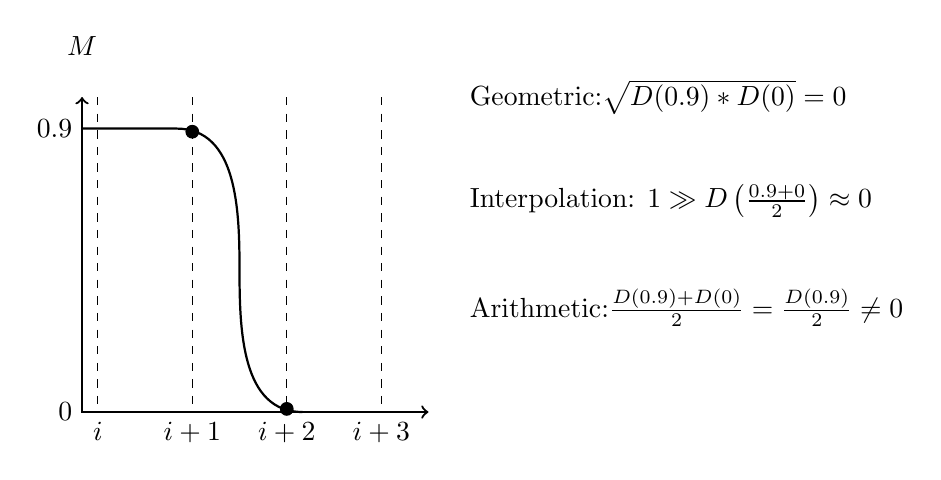
\begin{tikzpicture}[scale = 4]
    \draw[<->, thick] (1.1,0) -- (0,0) -- (0,1);
    \node[left] at (0,0.9) {$0.9$};
    \node[left] at (0,0) {$0$};
    \node[above] at (0,1.1) {$M$};

    \draw[thick] (0,0.9) -- (0.3,0.9) to [out=0,in=90] (0.5,0.45) to [out=270,in=180] (0.7,0.0);
    
    \draw[dashed] (0.35,1) -- (0.35, 0);
    \draw[dashed] (0.65,1) -- (0.65, 0);
    \draw[dashed] (0.05,1) -- (0.05, 0);
    \draw[dashed] (0.95,1) -- (0.95, 0);
    \node[below] at (0.05,0) {$i$};
    \node[below] at (0.35,0) {$i+1$};
    \node[below] at (0.65,0) {$i+2$};
    \node[below] at (0.95,0) {$i+3$};

    \draw[fill=black] (0.35,0.89) circle [radius=0.02];
    \draw[fill=black] (0.65,0.01) circle [radius=0.02];

    \node[right] at (1.2,1) {Geometric:$\sqrt{D(0.9)*D(0)}=0$};
    \node[right] at (1.2,0.67) {Interpolation: $1 \gg D\left(\frac{0.9+0}{2}\right) \approx 0$};
    \node[right] at (1.2,0.33) {Arithmetic:$\frac{D(0.9) + D(0)}{2} = \frac{D(0.9)}{2} \ne 0$};
  \end{tikzpicture}
  \caption{An illustration of the three methods for approximating the value of $D(M)$ at ghost points located in between the existing grid points.
    The two black circles represent the two points inconsideration for the calculations of geometric mean, interpolation of values, and arithmetic mean.
    The problem with Geometric mean is that $D(0)$ evaluates to $0$, resulting in no diffusion effects.
    With interpolation, the value of $D(0.45)$ is near-zero because $M \ll 1 \implies D(M) \approx 0$.
    For the arithmetic mean, since $D(0.9)$ is a larger value then the other methods some spatial diffusion actually work.
    }
  \label{fig:arithmeticMean}
\end{figure}

To simplify the spatial indexing, the grid functions are converted into vector functions by use of a bijective mapping defined as:
%!% l.378 ... your definition of \pi is not quite correct. you have {0,...,n} \times {0,...,m} i.e. you should have (n+1)*(m+1) grid points but your target sat {0,...,nm} has only n*m+1 point, so you are short m+1 grid points. ... also the function \pi as defined is not quite correct ... for example, for i=0 the second term is negative. i think what you mean is probably j+i*m
\begin{equation}
\begin{array}{c c c c}
  %!% Make sure this actually maps to {1, \ldots, nm} instead of 1.... (n+1)(m+1)
  \pi :& \{ 1, \ldots, n\} \times \{1, \ldots, m\} & \to & \{1, \ldots, nm \} \\
       & (i,j)                                     & \mapsto & \pi(i,j)
\end{array}
\end{equation}
%!% I have a figure for this?!?!?!?
Now, a single index can be used to iterate over the vector, $l$. 
Lexigraphical ordering is used here resulting in a bijective function $\pi(i,j) = j+ (i-1)m$.
This gives the system,
\begin{equation} \label{equ:M_space_discret}
  \frac{M^{k+1}_{l} - M^{k}_{l}}{\Delta t} =
    \frac{1}{\Delta x^2} \sum_{\sigma \in \mathcal{N}_{\pi^{-1}(l)}} \left(
    \left( \frac{D(M^{k+1}_{\pi(\sigma)}) + D(M^{k+1}_{l})}{2} \right)
    \cdot \left( M^{k+1}_{\pi(\sigma)} - M^{k+1}_{l} \right) \right)
    + F(C^{k+1}_{l}) M^{k+1}_{l}
\end{equation}
\begin{equation} \label{equ:C_space_discret}
  \frac{C^{k+1}_{l} - C^{k}_{l}}{\Delta t} = \frac{1}{2} ( G(C^{k+1}_{l}) M^{k+1}_{l} + G(C^{k}_{l}) M^{k}_{l} ).
\end{equation}

